\section{View}

  This chapter discusses the implementation of the features on the user interface described in \autoref{sub:design_view}.

  \subsection{Navigation}
  
    The user interface contains functionalities for several use cases, merged into a single web application. In a web application, routing plays a key role in determining what to show the user based on the URL address entered on the browser. Specifically in this case, routing can help in categorizing the current context of the application that consists of several views for different use cases. The following routes are implemented in the UI:

    \begin{itemize}
     \item Home page (path: \verb;/;)
     \item Create a new rule (path: \verb;/rules/new;)
     \item Edit a rule (path: \verb;/rules/<ruleName>;)\footnote{\emph{<ruleName>} refers to a dynamic value of a rule's name. Please take a look into \url{https://router.vuejs.org/guide/essentials/dynamic-matching.html} for more information.}
     \item List of rules (path: \verb;/rules;)
     \item Create a new validation (path: \verb;/validations/create;)
     \item See validation progress for specific validation ID (path: \verb;/validations/:validationId;)
     \item List of validations (path: \verb;/validations;)
    \end{itemize}
    
    To help the user in navigating the UI, a header is created and displayed on every page of the application. The header includes three buttons (\textsc{Home, Rules} and \textsc{Validations}), that links the user to the corresponding view of the application. 

    \begin{figure}[!ht]
     
\includegraphics[width=\textwidth]{images/ss_navigation.jpeg}
     \caption{Screenshot of the header to navigate the UI}
    \end{figure}

  \subsection{Rule Management Form}
  
    The rule management form is a reusable form, can be used to both create a new and edit an existing validation rule. The rule management form displays all the attributes of a \verb;ValidationRule; model as a form field. 

    \begin{figure}[!ht]
      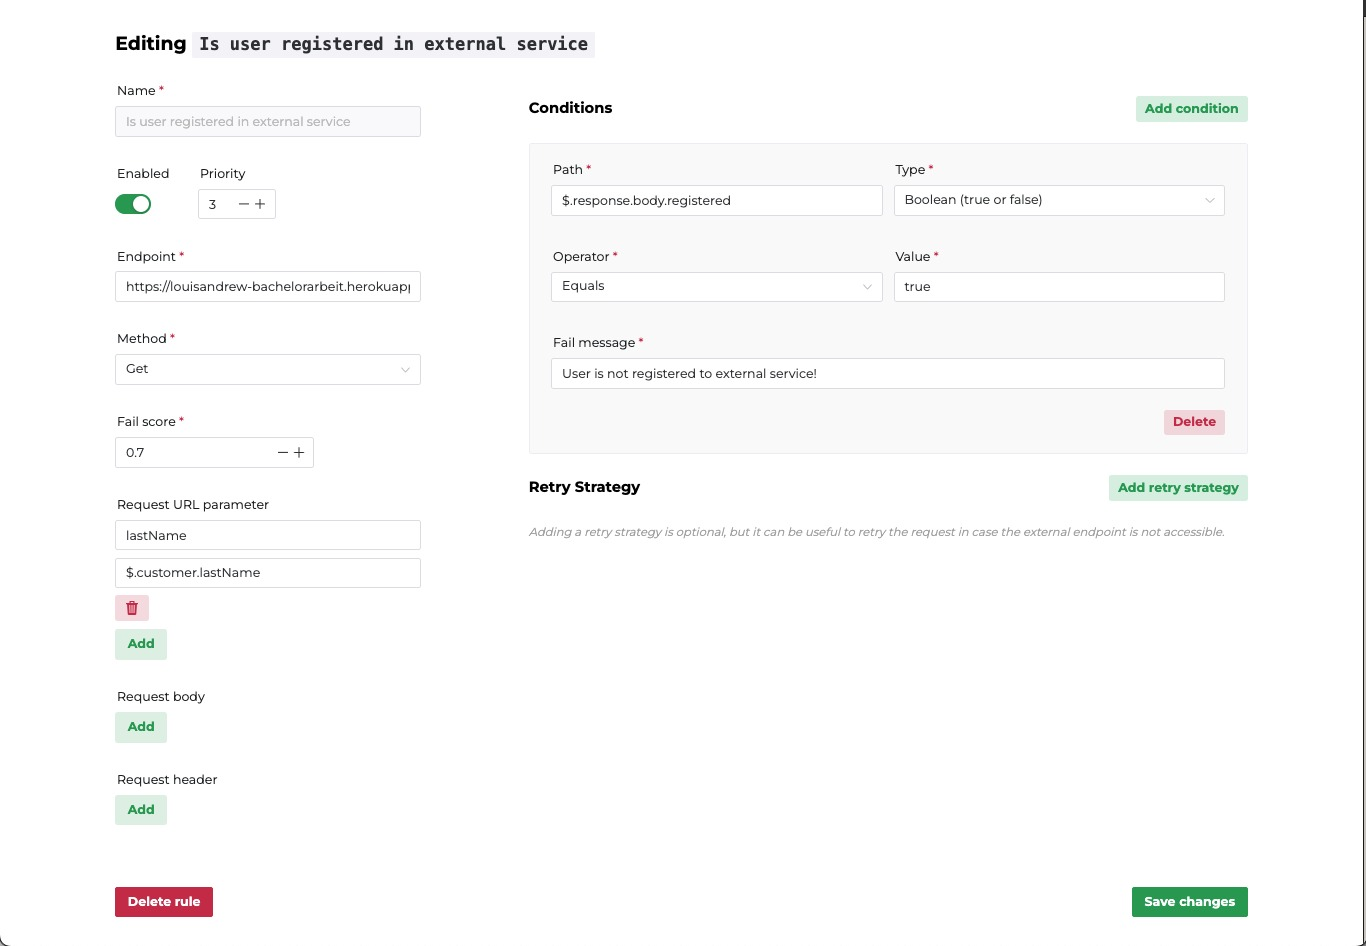
\includegraphics[width=\textwidth]{images/ss_sample_filled.jpeg}
      \caption{Screenshot of the rule management form}
    \end{figure}

    \subsubsection{Conditions Section}

      The \textsc{Conditions} section is a component, used to add one more condition to a validation rule. The \textsc{Conditions} section renders the list of conditions provided in a card, containing form fields for each attribute of the particular condition. Each card represents a single form, which also contains validation on its fields. 
      
      As mentioned before, the available values for the \verb;operator; attribute of a condition depends on its \verb;type; attribute. To prevent an invalid condition being sent to the FDS, the \textsc{Operator} field is a select field, and its options are defined by the current value inputted on the \textsc{Type} field. The intention of the restriction is to make sure that the \verb;operator; chosen is always valid to the corresponding \verb;type; of the condition.

      \begin{lstlisting}[style=es6, caption={Function to get list of available operators based on type (TypeScript)}]
const getAvailableOperators = (type: ConditionType) => {
  switch (type) {
    case "string":
      return [
        { label: "Equals", value: "eq" },
        { label: "Starts with", value: "starts" },
        { label: "Includes", value: "incl" },
        { label: "Ends with", value: "ends" },
      ]
    case "number":
      return [
        { label: "Greater than", value: "gt" },
        { label: "Greater than equals", value: "gte" },
        { label: "Lesser than", value: "lt" },
        { label: "Leser than equals", value: "lte" },
        { label: "Equals", value: "eq" },
      ]
    case "array":
      return [
        { label: "Includes", value: "incl" },
        { label: "Excludes", value: "excl" },
        { label: "Number of items equals", value: "len" },
        { label: "Is empty", value: "empty" },
      ]
    case "boolean":
      return [{ label: "Equals", value: "eq" }]
    default:
      return []
  }
}
      \end{lstlisting}

      \begin{figure}[!ht]
        \centering
        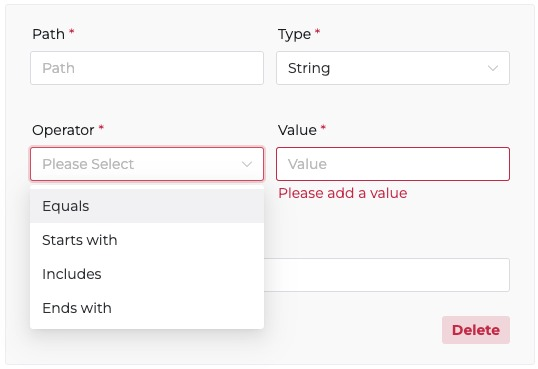
\includegraphics[width=0.8\textwidth]{images/ss_condition_op.jpeg}
        \caption{Screenshot of the "Operator" select field options, based on the current "Type" value}
      \end{figure}
      
      If more than one condition is provided, a radio field is also rendered, so that the user can choose one of the provided modifier for the list of conditions (either \textbf{\emph{ALL}} or \textbf{\emph{ANY}}). 

      A form validation is also implemented in the \textsc{Conditions} section. The validation not only make sure that all the required fields are filled, but also the value of the fields itself. For example, the validation will display an error message if the \textsc{Type} field is set to "Number", but the input value of the \textsc{Value} field is not a valid number. 

    \subsubsection{Autocomplete Input}

    A JSONPath expression is a valid value for some attributes of a \verb;ValidationRule;, and it also might be needed to access the current runtime information during a validation process, such as the HTTP response from the external endpoint, runtime secrets and customer information. Unfortunately, it might be difficult to memorize the expressions needed to access certain values, and it might also confuse the user. 

    \begin{figure}[!ht]
      \centering
      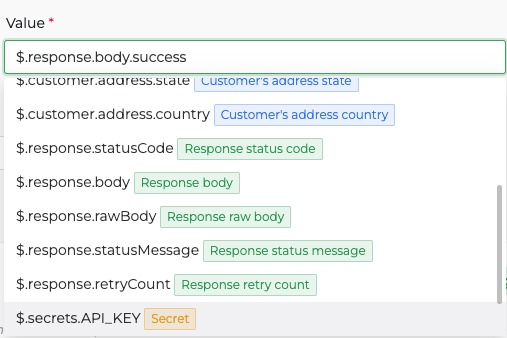
\includegraphics[width=0.5\textwidth]{images/ss_autocomplete.jpeg}
      \caption{Screenshot of the autocomplete input usage}
    \end{figure}

    To solve this problem, an autocomplete input field is provided in certain fields where a JSONPath expression is used. User can then display a list of possible JSONPath expressions by prefixing an input field with "\$", and choosing one of the expressions listed. User can also extend the expression chosen. The autocomplete input is used in the following form fields:

    \begin{itemize}
      \item \textsc{Path} field on \textsc{Conditions} section
      \item \textsc{Value} field on \textsc{Conditions} section
      \item Value field of a dynamic input\footnote{Autocompletion on \emph{\$.response} is not available here.}
    \end{itemize}

  \subsection{Validation Form}

  \subsection{Validation Progress}
  
  \subsection{Rule List and Validation List}